% ---
% school: "college"
% level: "8eme"
% section: null
% chapter: "التناظر المركزي"
% source: "Axiomaths"
% title: "تركيب : مثلث قائم ومناظراته"
% country: "Tunisie"
% year: 2026
% professor: "Axiomaths"
% difficulty: "Moyen"
% points: null
% tags: ["symetrie-centrale", "symetrie-axiale", "angles", "rectangle", "synthese"]
% ---
% Exercice 9/19 de la série 8ème « التناظر المركزي » (statement + \axsol + solution). Compiler avec XeLaTeX + axiomath.sty (+ axiomaths-logo.png).
\documentclass[12pt,a4paper]{article}
\usepackage[level=8b,color=15803D]{axiomath}
\usetikzlibrary{arrows.meta}
\newcommand{\cm}{\,\mathrm{cm}}
\axsetup{title={التناظر المركزي}, corrige}

\begin{document}

\begin{corr}[title={تركيب : مثلث قائم ومناظراته}, stars=3, source={Axiomaths}]
$ABC$ مثلث قائم الزاوية في $A$ حيث $AB=4\cm$ و $\widehat{ABC}=35^\circ$. $I$ منتصف $[BC]$ ، $D$ مناظرة $A$ بالنسبة إلى $I$ ، و $E$ مناظرة $C$ بالنسبة إلى المستقيم $(AB)$.
\begin{enumerate}
  \item ابنِ الشكل ثم احسب $\widehat{ACB}$.
  \item بين أن $A$ منتصف $[CE]$.
  \item بين أن $BE=BC$ ثم احسب $\widehat{EBC}$.
  \item ما طبيعة المثلث $BCE$ ؟ احسب $\widehat{BEC}$.
  \item بين أن $ABDC$ مستطيل ثم أن $AD=BE$.
\end{enumerate}
\axsol
\begin{enumerate}[itemsep=14pt]
  \item\leavevmode
  \begin{prop}[مجموع زوايا مثلث]
  مجموع قيس زوايا مثلث يساوي \ib{$180^\circ$}.
  \end{prop}
  في المثلث $ABC$ : $\widehat{ACB}=180^\circ-90^\circ-35^\circ=55^\circ$.
  \begin{center}
  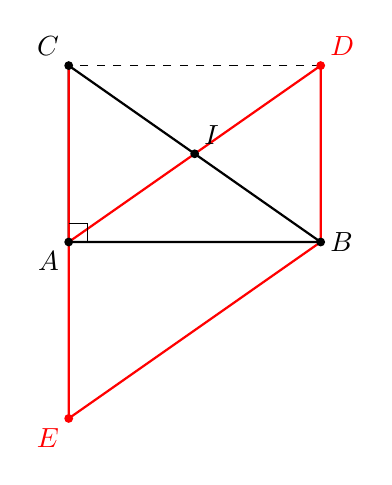
\begin{tikzpicture}[scale=0.8]
    \draw[thick] (0,0)--(4,0)--(0,2.8008)--cycle;
    \draw[thick,red] (0,2.8008)--(0,-2.8008)--(4,0);
    \draw[thick,red] (0,0)--(4,2.8008)--(4,0);
    \draw[dashed] (4,2.8008)--(0,2.8008);
    \draw (0,0.3)--(0.3,0.3)--(0.3,0);
    \fill (0,0) circle (2pt) node[below left] {$A$};
    \fill (4,0) circle (2pt) node[right] {$B$};
    \fill (0,2.8008) circle (2pt) node[above left] {$C$};
    \fill[red] (0,-2.8008) circle (2pt) node[below left] {$E$};
    \fill[red] (4,2.8008) circle (2pt) node[above right] {$D$};
    \fill (2,1.4004) circle (2pt) node[above right] {$I$};
  \end{tikzpicture}
  \end{center}
  \item $E$ مناظرة $C$ بالنسبة إلى $(AB)$ ، إذن $(AB)$ هو محور القطعة $[CE]$ : $(AB)\perp(CE)$ ، و $(AB)$ يمر من منتصف $[CE]$.
  بما أن $(AC)\perp(AB)$ أيضا، فالمستقيمان $(AC)$ و $(CE)$ المارّان من $C$ والعموديان على $(AB)$ منطبقان : $E\in(AC)$.
  منتصف $[CE]$ ينتمي إلى $(AB)$ وإلى $(AC)$ ، أي هو $A$. إذن \ib{$A$ منتصف $[CE]$}.
  \item $B$ تنتمي إلى المحور، فمناظرتها هي $B$ نفسها. و $S_{(AB)}$ يحوّل $C$ إلى $E$ ، فهو يحفظ الأطوال :
  \[BE=BC\]
  التناظر المحوري يحفظ قيس الزوايا، فـ $\widehat{EBA}=\widehat{CBA}=35^\circ$. و $E$ و $C$ على جهتين مختلفتين من $(AB)$ ، إذن :
  \[\widehat{EBC}=\widehat{EBA}+\widehat{ABC}=35^\circ+35^\circ=70^\circ\]
  \item $BE=BC$ ، فالمثلث $BCE$ \ib{متقايس الضلعين} رأسه $B$. زاويتا القاعدة متقايستان :
  \[\widehat{BEC}=\widehat{BCE}=\dfrac{180^\circ-70^\circ}{2}=55^\circ\]
  وهذا متفق مع $\widehat{ACB}=55^\circ$ لأن $E$ تنتمي إلى $(AC)$.
  \item قطرا $ABDC$ هما $[AD]$ و $[BC]$. $I$ منتصف $[BC]$ ، و $I$ منتصف $[AD]$ لأن $D=S_I(A)$. للقطرين نفس المنتصف، فالرباعي $ABDC$ متوازي أضلاع.
  زاويته في $A$ قائمة، إذن هو \ib{مستطيل}. وقطرا المستطيل متقايسان : $AD=BC$.
  ومن السؤال 3 : $BE=BC$. إذن \ib{$AD=BE$}.
\end{enumerate}
\textbf{الفكرة :} $A$ هي في نفس الوقت منتصف $[CE]$ وعلى محور التناظر : التناظران المحوري والمركزي يتقاطعان في هذا الشكل.
\end{corr}

\end{document}
